\documentclass[a4paper, 12pt]{article}

%Paragraph jumps and indentation
\setlength{\parskip}{1.5em}
\setlength{\parindent}{1.25cm}

%Border
\usepackage[left=1in, right=1in, top=1in, bottom=1in]{geometry}

%Double spacing
\usepackage{setspace}
\doublespacing

%Packages
\usepackage{amsmath}
\usepackage[dvipsnames]{xcolor}
\usepackage{mathtools}
\usepackage{amsfonts}
\usepackage{titlesec}

%Images
\usepackage{graphicx}
\graphicspath{ {./images/} }
\usepackage{wrapfig}
\usepackage{float}
\usepackage{caption}

%Tables
\usepackage{multirow}
\usepackage{array}
\usepackage{tabu}
\titleformat{\section}
{\normalfont\large\bfseries}{\thesection}{1em}{}
\titleformat{\subsection}
{\normalfont\large\bfseries}{\thesubsection}{1em}{}

%Equation numbering
\counterwithin{equation}{section}

%Links
\usepackage{hyperref}
\urlstyle{same}

%Diagrams
\usepackage{pgfplots}
\pgfplotsset{compat=newest}
\usetikzlibrary{positioning, arrows.meta}
\usepgfplotslibrary{fillbetween}
%\tikzset{every node/.style={font=\small}}


\begin{document}

\begin{titlepage}
  \begin{center}
    \textbf{IB ECONOMICS} \hspace{1cm} STANDARD LEVEL\\
    \vspace*{3cm}
    \textbf{Title of the article:}
    Mozambique approves investment projects
    valued at about US\$5 billion in H1 2025\\

    \textbf{Source of the article:}
    African Mining Market\\

    \textbf{Link to the article:}
    \url{https://africanminingmarket.com/mozambique-approves-investment-projects-valued-at-about-usd5-billion-in-h1-2025}\\

    \textbf{Article publish date:}
    September 1, 2025\\

    \textbf{Article access date:} September 11, 2025\\

    \textbf{Commentary writing date:} \today\\

    \textbf{Unit of the syllabus:}
    Macroeconomics\\

    \textbf{Key concept:}
    Intervention.\\

    \vfill
    Word count: 772
  \end{center}
\end{titlepage}

\section*{Extract}
{ \itshape
  {\large The Mozambican government has approved 115 investment projects valued at about US\$5 billion in the first half of 2025, with the potential to create 17,000 jobs. Prime Minister Benvinda Levi announced the figures on 30th August, at the closing of the 60th Maputo International Fair (FACIM).}

  The largest project is Green Energy Mozambique, a US\$3 billion industrial park in Sofala province. The complex is expected to generate 10,000 direct jobs and boost production of key materials including aluminum, steel, cement, batteries, and solar panels.

  More than 88\% of total investment was directed to Sofala, far ahead of Maputo. Foreign capital accounted for US\$3.2 billion, with contributions from investors in 25 countries. The funds mainly target industry, transport, communications, and services. Domestic investment stood at US\$144 million.

  Levi said the results show the Mozambican economy is rebounding after climate shocks and post-election tensions, with the private sector driving growth. She also highlighted the launch of a US\$250 million mutual guarantee fund during the fair to support recovery and expand private sector participation.

  These achievements align with the country's strategy to strengthen investor appeal. In recent years, Mozambique has pursued reforms to attract capital, including the creation of the Investment and Export Promotion Agency (APIEX) and the adoption of a new investment law in 2023. The country now offers tax and customs incentives, along with special economic zones in agriculture, aquaculture, and less-developed regions.

  According to UNCTAD, Mozambique ranked fourth in Africa for foreign direct investment inflows in 2024, reaching US\$3.55 billion, up from US\$2.5 billion in 2023, when it placed sixth.

}

\newpage
\section*{Commentary}

In summary, Mozambique has approved major new investment projects worth about 5 billion USD, mostly foreign-funded and centered in Sofala, including a large green energy park producing important commodities.
The initiatives are expected to create jobs and support the country's economic recovery after recent shocks, with reforms and incentives aimed at strengthening investor confidence.
This commentary will discuss how indirect \textbf{intervention} by the government, in the act of facilitating and approving such projects, achieves its effects on increasing economic growth and decreasing unemployment.
The analysis shall be done with respect to the Keynesian model of aggregate demand (AD) and aggregate supply (AS).

Firstly, the immediate effect of approving `investment projects valued at about US\$5 billion' likely causes economic growth, and thereby alleviates the potential contraction caused by recent shocks.
This development represents direct investment spending.
As a component of GDP, an increase in investment spending directly increases aggregate demand.
\vspace{-2em}\begin{wrapfigure}{L}{0.48\textwidth}
  \begin{center}
    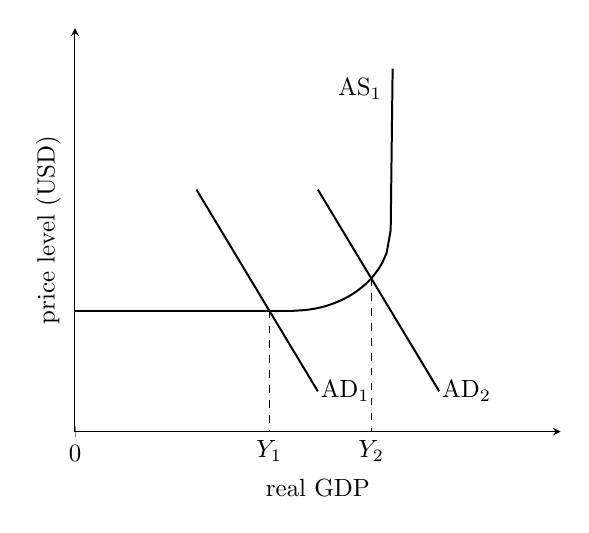
\begin{tikzpicture}[scale=0.9]
      \begin{axis}[
          axis lines=left,
          xlabel={real GDP},
          ylabel={price level (USD)},
          xmin=0, xmax=1,
          ymin=0, ymax=1,
          xtick={0}, ytick={\empty},
          clip=false
        ]

        \addplot[thick, domain=0:0.45] {0.3};
        \addplot[thick, domain=0.45:0.65] {0.5 - sqrt(1/25 - (x-0.45)^2)};
        \addplot[thick, domain=0.65:0.654] {100*x - 64.5};
        \node[left] at (0.65, 0.85) {AS$_1$};

        \addplot[thick, domain=0.25:0.5] {1.1-2*x};
        \node[xshift=11pt] at (0.5, 0.1) {AD$_1$};

        \addplot[thick, domain=0.5:0.75] {1.6-2*x};
        \node[xshift=11pt] at (0.75, 0.1) {AD$_2$};

        \draw[dashed] (0.4, 0.3) -- (0.4, 0);
        \node[below] at (0.4, 0) {$Y_1$};

        \draw[dashed] (0.61, 0.38) -- (0.61, 0);
        \node[below] at (0.61, 0) {$Y_2$};

      \end{axis}
    \end{tikzpicture}
    \captionsetup{
      justification=centering,
      font=small,
      labelfont=small
    }
    \caption{The short-run effect of increased investment on aggregate demand.}
  \end{center}
\end{wrapfigure}

\noindent It is reasonable to treat the `climate shocks and post-election tensions' in Mozambique as a source of a recessionary gap, manifest as insufficient aggregate demand.
According to the Keynesian model, an economy experiencing a recessionary gap cannot self-correct, so the government must act to boost aggregate demand. 
Although the 5 billion USD counts as investment spending in national accounts, the government's role in approving these projects makes the policy an indirect form of \textbf{intervention}.

In \textbf{Figure 1}, the initial aggregate demand is denoted by AD$_1$.
Following the 5 billion USD investment, aggregate demand increases to AD$_2$.
The recessionary gap is depicted with the initial demand curve AD$_1$ intersecting the Keynesian aggregate supply curve AS$_1$ at its flat portion, resulting in real GDP of $Y_1$.
The increase in aggregate demand to AD$_2$ increases real GDP to $Y_2$ with little effect on the price level, and the new intersection is on the upwards sloping part of the supply curve.
This aligns with Keynesian theory and indicates short-run economic growth.
Such a noticeable increase in AD is reasonable to assume, considering that 5 billion USD is a significant amount of money compared to Mozambique's GDP in September 2025, which is 22.44 billion USD.

\vspace{-2em}\begin{wrapfigure}{L}{0.48\textwidth}
  \begin{center}
    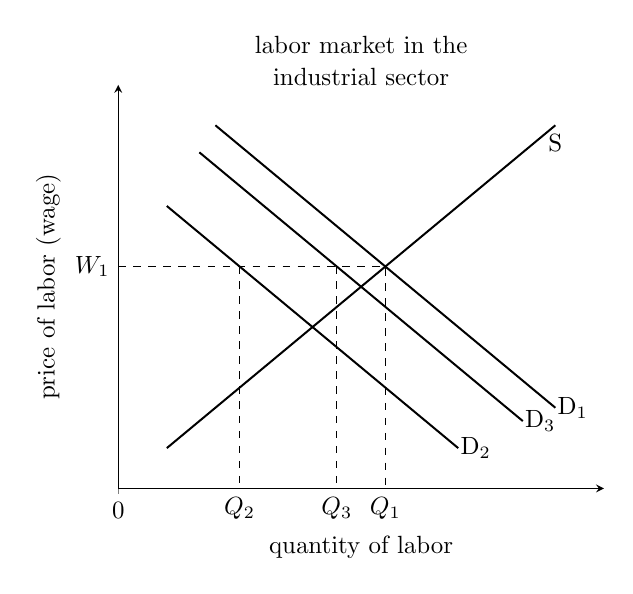
\begin{tikzpicture}[scale=0.9]
      \begin{axis}[
          axis lines=left,
          xlabel={quantity of labor},
          ylabel={price of labor (wage)},
          y label style={at={(axis description cs:-0.1,.5)},anchor=south},
          xmin=0, xmax=1,
          ymin=0, ymax=1,
          xtick={0}, ytick={\empty},
          clip=false
        ]

        \node at (0.5, 1.1) {labor market in the};
        \node at (0.5, 1.02) {industrial sector};
        
        \addplot[thick, domain=0.1:0.9] {x};
        \addplot[thick, domain=0.1:0.7] {0.8 - x};
        \addplot[thick, domain=0.2:0.9] {1.1- x};
        \addplot[thick, domain=0.167:0.833] {1- x};
        \node[below] at (0.9, 0.9) {S};
        \node[xshift=7pt] at (0.9, 0.2) {D$_1$};
        \node[xshift=7pt] at (0.7, 0.1) {D$_2$};
        \node[xshift=7pt] at (0.833, 0.167) {D$_3$};
        
        \draw[dashed] (0, 0.55) -- (0.55, 0.55) -- (0.55, 0);
        \node[below] at (0.55, 0) {$Q_1$};
        \node[left] at (0, 0.55) {$W_1$};

        \draw[dashed] (0.25, 0.55) -- (0.25, 0);
        \node[below] at (0.25, 0) {$Q_2$};


        \draw[dashed] (0.45, 0.55) -- (0.45, 0);
        \node[below] at (0.45, 0) {$Q_3$};

      \end{axis}
    \end{tikzpicture}
    \captionsetup{
      justification=centering,
      font=small,
      labelfont=small
    }
    \caption{Increase in demand of labor}
  \end{center}
\end{wrapfigure}

\noindent In addition to an immediate increase in investment spending, it is likely that there is also more consumer spending, contributing to aggregate demand.
The creation of 10,000 direct jobs in the industrial sectors increases household income, and reducing cyclical unemployment.

In \textbf{Figure 2}, D$_1$ represents the demand of labor in the Mozambican industrial sector before these shocks, which reduce its demand to D$_2$.
Keynesian theory claims that wages are inflexible downwards, so the wage remains at $W_1$, resulting in cyclical unemployment of $Q_1 - Q_2$.
The effect of the newly created jobs is shown as an increase in demand, from D$_2$ to D$_3$, which works to lessen unemployment to $Q_1 - Q_3$.
More employment means more household income, so consumer spending is increased.

These investment projects also have a long-run effect on aggregate demand.
The increased output from these industries allows for the export of a portion of the commodities produced in this industrial park.
This is likely, given that most of the investment originates from foreign sources.



\begin{wrapfigure}{L}{0.48\textwidth}
  \begin{center}
    \begin{tikzpicture}[scale=0.9]
      \begin{axis}[
          axis lines=left,
          xlabel={real GDP},
          ylabel={price level (USD)},
          xmin=0, xmax=1,
          ymin=0, ymax=1,
          xtick={0}, ytick={\empty},
          clip=false
        ]

        \addplot[thick, domain=0:0.55] {0.3};
        \addplot[thick, domain=0.55:0.75] {0.5 - sqrt(1/25 - (x-0.55)^2)};
        \addplot[thick, domain=0.75:0.754] {100*x - 74.5};
        \node[right] at (0.75, 0.85) {AS$_2$};

        \addplot[thick, domain=0.45:0.65] {0.5 - sqrt(1/25 - (x-0.45)^2)};
        \addplot[thick, domain=0.65:0.654] {100*x - 64.5};
        \node[left] at (0.65, 0.85) {AS$_1$};
      \end{axis}
    \end{tikzpicture}
    \captionsetup{
      justification=centering,
      font=small,
      labelfont=small
    }
    \caption{The long-run effect of job creation and infrastructure on aggregate supply.}
\end{center}
\end{wrapfigure}
\noindent The investment in physical capital, such as establishing Green Energy Mozambique in Sofala, also improves potential output, creating long term economic growth.
With more production of key commodities such as aluminum, steel, cement, batteries, and solar panels, the amount of output supplied at any given price level is increased.
In other words, the aggregate supply in the Mozambican economy increases.

The increase is illustrated in \textbf{Figure 3}, with AS$_1$ same as in \textbf{Figure 1}, and AS$_2$ corresponding to the increased aggregate supply following this change.
As the figure shows, it is now possible to create a higher amount of real output without significantly increasing the price level.
This indicates long-term economic growth in the economy.

This increase in aggregate supply also reflects a market-based supply-side intervention. 
The creation of Green Energy Mozambique supports sustainable production.
By improving efficiency and limiting the external costs of pollution and resource depletion, the project helps ensure that the economy can maintain high levels of output in the future.

The effects of \textbf{intervention} ideally increase AD in the short run and pull the economy out of contraction.
In the long run increases in AD, caused by increased consumption spending and net exports, and
increases in AS, caused by capital improvements and incentives to improve long-term efficiency.
All these improvements combined mean it is reasonable to expect more economic growth in Mozambique in the future, if climate shocks and political tensions can be successfully avoided.

\end{document}